\documentclass[12pt,notitlepage,nofootinbib]{revtex4}
\usepackage{graphicx}
\usepackage{bm}
\usepackage{rotating}
\def\baselinestretch{1.2}
\usepackage{dcolumn}
\usepackage{times}
\usepackage{color}
\usepackage{amsmath} 
\usepackage{extarrows}
\usepackage{listings}
\usepackage{url}
\setlength{\mathindent}{0pt}

\begin{document}

\title{StochSS Hands-on Tutorial Series: 1 - Basic Introduction to StochSS (non-spatial stochastic modeling)}

\author{StochSS Development Team}
\affiliation{Department of Computer Science - University of California, Santa Barbara}

\date{\today}

\maketitle

This tutorial will guide you through the basic features of StochSS. You will become familiar with the \textbf{Model Editor} and with the \textbf{Simulation Manager}. You will learn how to create your own model, which can be \textit{population or concentration-based}, and how to simulate it, locally or in the cloud, using either an ordinary differential equation (ODE) solver or the stochastic simulation algorithm (SSA).
More advanced StochSS features such as sensitivity analysis for ODE models, parameter estimation for mass action-based, non spatial stochastic models, and spatial stochastic solvers are covered in other tutorials.

\section{\label{sec:pre}Prerequisites}
\begin{itemize}
\item StochSS 1.4 (or later) installed on your computer (please follow download and installation instructions at \url{www.stochss.org}). 
\item A basic understanding of well-mixed discrete stochastic simulations and models based on ordinary differential equations \cite{dan,sundials}. 
\item The following admin login screen appears in your browser:
\end{itemize}

\begin{figure}[!htb]
\centering
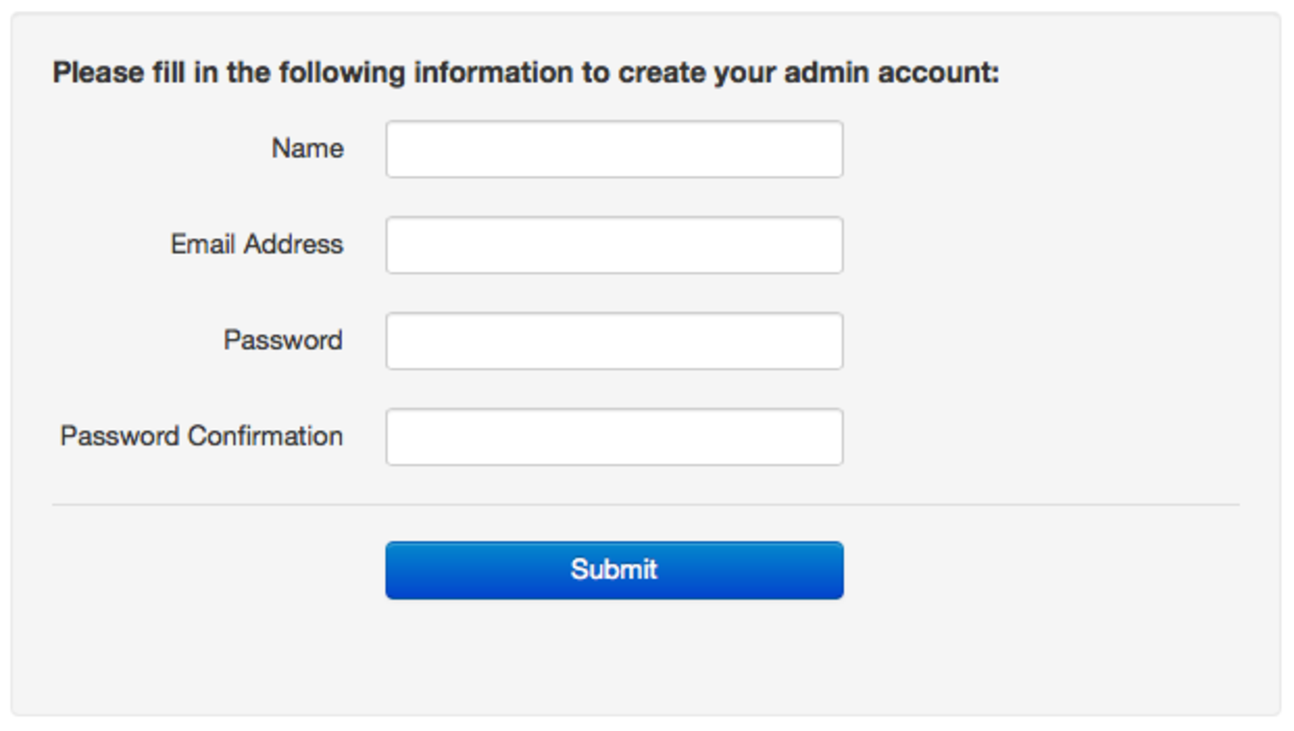
\includegraphics[scale=0.64]{admin-login.pdf}
\caption{Administrator login page}
\end{figure}

\section{\label{sec:acc} Creating Administrator and Standard User Accounts}
The new user authentication system is currently set up to operate with \textbf{one} admin user and any number of regular users. At the end of a successful installation process, your default browser will launch the StochSS server and a new admin login page will open. You will be asked to create an \textbf{admin account}. Once the admin account is created you will be forwarded to a regular login page (Fig.~\ref{fig:1}) where the admin and the approved users can enter the StochSS GUI. The regular login page also allows regular users to request an account. The admin user has access to the \textcolor{blue}{`Admin Panel'}, which has three tables: one for displaying all of the active user accounts in the system (\textcolor{blue}{`Active Users�} table), one for displaying all of the email addresses of the users who have been approved and haven�t created their account yet (\textcolor{blue}{`Approved Users�} table), and one for displaying all of the email addresses of the users who have requested accounts and not yet been approved (\textcolor{blue}{`Users Awaiting Approval�} table). The approved users table allows the admin to delete active users, as well as reset their passwords.

\begin{figure}[!htb]
\centering
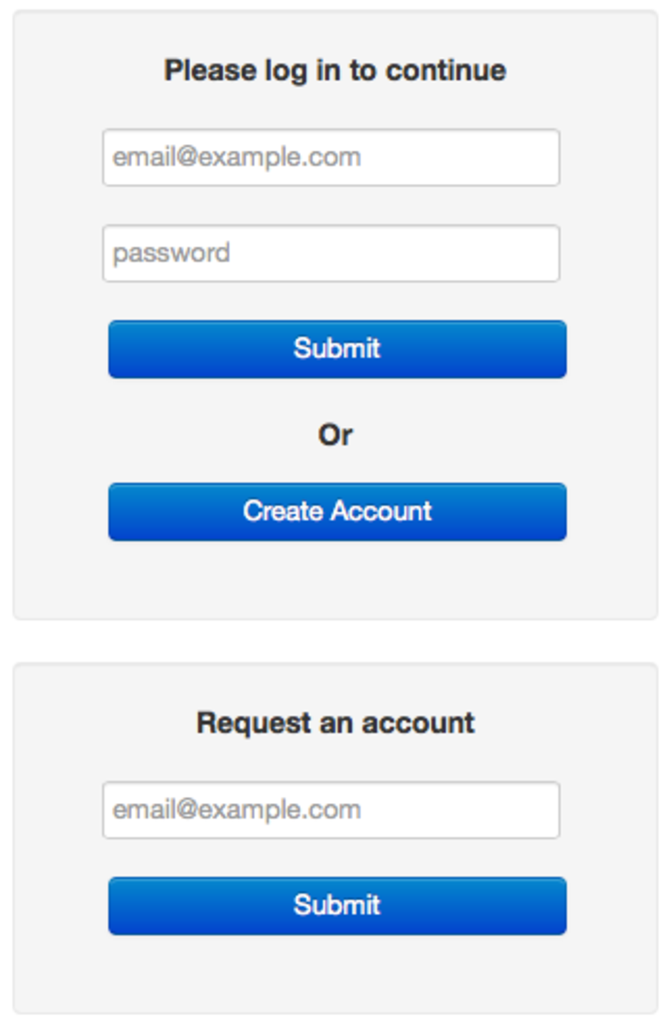
\includegraphics[scale=0.64]{user-login.pdf}
\caption{User login page}
\label{fig:1}
\end{figure}

\section{\label{sec:imp} Importing a Model}
The \textbf{model editor} will let you create new or modify existing well-mixed stochastic biochemical models as well as deterministic models based on ODEs. The easiest way to get started using the \textbf{model editor} is to import an example model, and then to browse the different tabs.

\subsection{Importing an existing StochKit2 model (population model)}
\underline{Option 1}
\begin{itemize}
  \item \textbf{Navigate} to the main \textcolor{blue}{Model editor} page.
  \item \textbf{Select} the menu \textcolor{blue}{\textit{`Import $>$ From File'}}.
  \item \textbf{Enter} a model name in the \textcolor{blue}{\textit{Name}} text box.
  \item \textbf{Select} an XML file. A collection of example models can be found in the directory \textcolor{blue}{\textit{examples}} within the \textcolor{blue}{\textit{StochSS}} native folder.
  \item \textbf{Click} on the \textcolor{blue}{`Import'} button.
\end{itemize}

\underline{Option 2}
\begin{itemize}
  \item \textbf{Navigate} to the main \textcolor{blue}{Model editor} page.
  \item \textbf{Select} the menu \textcolor{blue}{\textit{`Import $>$ Public Library'}}.
  \item \textbf{Select} a model from the Public Library \textbf{clicking} on \textcolor{blue}{Import}.
  \item \textbf{A pop-up window} will appear on your screen allowing you to name your model and confirm.
\end{itemize}

To verify that the model import was successful, navigate back to the \textcolor{blue}{Model editor} page. At this point we suggest you \textbf{explore} the different tags in the \textcolor{blue}{Model editor} to become familiar with the \textbf{StochSS GUI} and to take a look at how the different \textit{Species}, \textit{Parameters} and \textit{Reactions} are defined.

\subsection{Importing an existing StochKit2 Model (concentration-based model)}
StochSS now supports both population and concentration-based models. Concentration-based models are imported the same way as population-based models.
It is important to notice at this point that, when the concentration-based model is created and selected, a link to the \textcolor{blue}{concentration-to-population conversion} page appears on the right side of the screen (\textcolor{blue}{Convert to Population}).

\subsection{Converting a concentration model to population}
\begin{itemize}
  \item \textbf{Click} on the \textcolor{blue}{`Convert to Population'} item on the right to start the conversion process. The model conversion page will open.
  \item \textbf{Click} on the \textcolor{blue}{`Create Model'} button at the bottom right of the page to create a population-based model. This newly created population model can be simulated using both deterministic and stochastic solvers.
\end{itemize}

\textcolor{red}{\textbf{The conversion process operates correctly only if the model to be converted is entirely based on \textcolor{blue}{mass action kinetics}. If the model to be converted is \textcolor{blue}{NOT} entirely based on mass action kinetics, the conversion tool only scales the concentrations to population (integer) values, without modifying the rates (parameters).}}

\section{Creating a New Model}
As a representative example, we use the \textcolor{blue}{dimer-decay} population model defined by the following four reactions:
\[ \begin{cases}
S1 + S1 \xlongleftrightarrow[\leftarrow c3]{c2\rightarrow} S2 \xlongrightarrow{c4} S3 \nonumber \\
S1 \xrightarrow{c1} \emptyset. \nonumber
\end{cases} \]
The creation of a new model using the \textcolor{blue}{Model editor} progresses through the following steps:
\begin{itemize}
\item \textbf{Navigate} to the main \textcolor{blue}{Model editor} (the \textcolor{blue}{`Model'} tag is selected by default).
\item \textbf{Type in} a model name in the \textcolor{blue}{`Name'} text box, select the \textcolor{blue}{`Population'} button and the  \textcolor{blue}{`Non-spatial'} button. Finally, \textbf{click} on the \textcolor{blue}{`Create model'}  button.
 \item \textbf{Click} on the \textcolor{blue}{`Species�} tag to define chemical species names and their initial values (number of molecules in this case). 
 \item \textbf{Use} the \textcolor{blue}{`Add species�} button on the right to add \textit{S1}, \textit{S2} and \textit{S3} species with initial populations of $10000, 0, 0$, respectively.
 \item \textbf{Click} on the \textcolor{blue}{`Parameters�} tag to define the model parameters' names and their expressions. 
 \item \textbf{Use} the \textcolor{blue}{`Add parameter�} button to add parameters \textit{c1, c2, c3} and \textit{c4} and their values $1.0, 0.002, 0.5$ and $0.04$, respectively.
 \item \textbf{Click} on the \textcolor{blue}{`Reactions�} tag to define reaction names, reactants, products and propensities.
 \item \textbf{Use} the \textcolor{blue}{`Add reaction�} button to add reactions \textit{R1, R2, R3, R4} (see Fig.~\ref{fig:2}).
\end{itemize}

\begin{figure}[!htb]
\centering
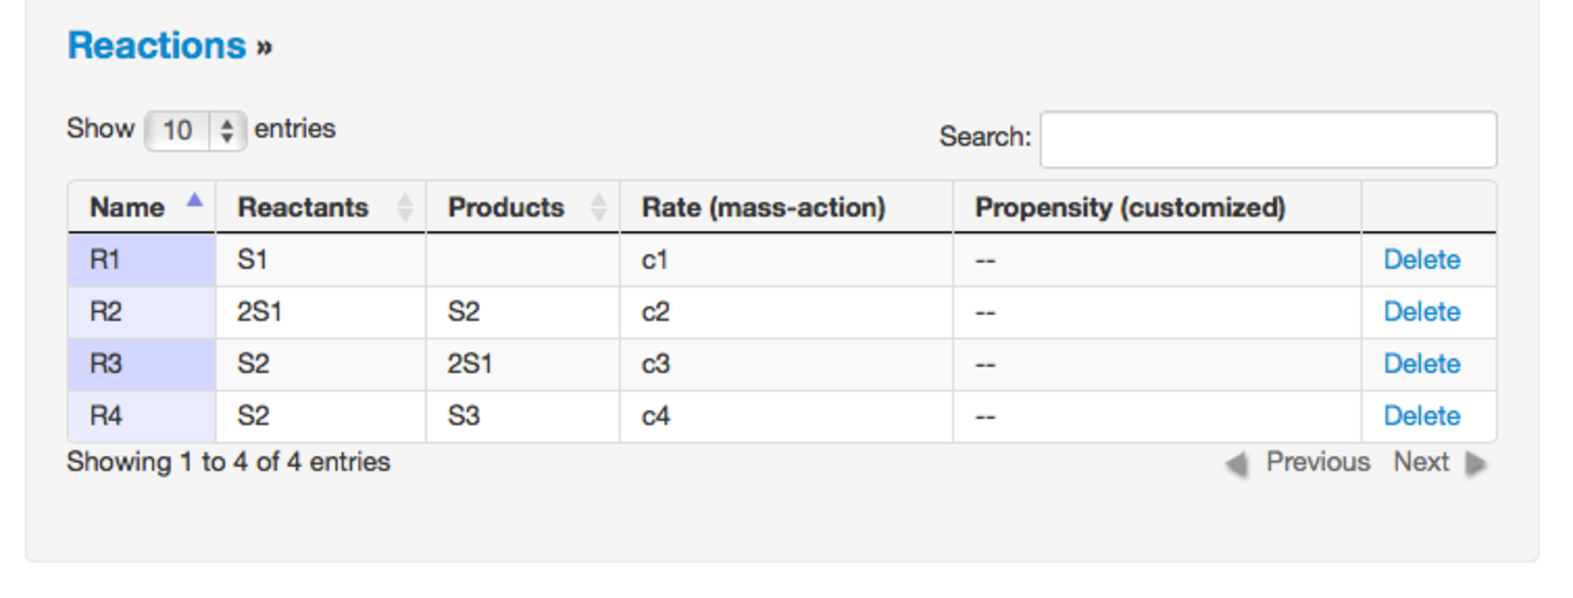
\includegraphics[scale=0.64]{reactions.pdf}
\caption{Reactions page}
\label{fig:2}
\end{figure}

\section{Cloud Computing}
You can also use Amazon Elastic Compute Cloud (EC2) to execute your simulation jobs. Using the cloud for your simulation deployments requires that you set up an \textcolor{blue}{Amazon Web Services (AWS)} account and download your AWS credentials.
\subsection{Sign up for an Amazon Web Services account (if you do not already have one).}
\begin{itemize}
\item \textbf{Navigate} to \url{http://aws.amazon.com} and click the \textcolor{blue}{`Sign Up�} button.
\item An Amazon Web Services (cloud) account requires that you put in credit card information. Amazon will charge for the cloud resources you use via the StochSS app. StochSS automatically shuts down all instances that have been inactive for 2 hours.
\item Amazon Micro server instance pricing:\\
 \url{http://aws.amazon.com/ec2/pricing/#on-demand}.
\item Amazon standard storage pricing (for job results):\\
\url{http://aws.amazon.com/s3/pricing}
\end{itemize}
\subsection{Download and save your EC2 credentials}
\begin{itemize}
\item \textbf{Navigate} to \textit{http://aws.amazon.com} and select \textbf{Security Credentials} from the \textcolor{blue}{`My Account / Console�} menu next to the \textcolor{blue}{`Sign Up�} button.
\item \textbf{Click} the $+$ next to \textcolor{blue}{`Sign Up'} button.
\item \textbf{Click} \textcolor{blue}{`Create New Root Key'}. This process asks you to download and save a file called \textcolor{blue}{\textit{rootkey.csv}}. Store this file in a safe place. If you lose it, you will have to delete the access key and start again with a new set.
\item \textbf{Sign out} of the AWS Console by selecting \textcolor{blue}{`Sign Out�} from the drop down menu under your name at the top of the page.
\end{itemize}

\section{Running a Simulation}

\subsection{Locally}
\begin{itemize}
\item You can use your local machine (the one on which you deploy and run StochSS) to execute
your simulation jobs. \footnote{For Windows users, Amazon EC2 is required. Local execution is not supported at the moment.}
\item \textbf{Navigate} to the \textcolor{blue}{Simulation manager} page.
\item \textbf{Select} the model you wish to simulate and \textbf{click} on the \textcolor{blue}{`Next�} button. If you are trying to simulate a population-based model you can choose between the deterministic and the stochastic solver. If you choose the deterministic solver, you have the possibility to perform sensitivity analysis on a set of chosen parameters related to your model. Concentration-based models, on the other hand, can only be simulated using the deterministic solver.
\item \textbf{Setup} your simulation parameters: name, time, data storage frequency, realizations and solver type. 
\item The default stochastic solver is SSA. To use tau-leaping instead and to define the initial random seed, \textbf{click} on \textcolor{blue}{`Advanced Settings�}.
\item \textbf{Click} on the \textcolor{blue}{`Run locally� button'}. We suggest that you only run small jobs on machines with limited resources.
\item \textbf{Navigate} to the \textcolor{blue}{Job Status} page to check the status of your simulation.
\item \textbf{Click} on the \textcolor{blue}{`View results�} link to open the \textcolor{blue}{Job summary} page where you can plot the simulation�s trajectories and download the simulation�s output files.
\end{itemize}

\subsection{In the cloud}
\textbf{Extract your EC2 credentials from the downloaded file.}
\begin{itemize}
\item Open the \textcolor{blue}{\textit{rootkey.csv}} file downloaded following the instructions above. You can use a text editor to do so. The file contains two lines:\\
\textcolor{blue}{AWSAccessKeyId}=XXXXXXXXXXXXXXXXXXXXXX \\
\textcolor{blue}{AWSSecretKey}=YYYYYYYYYYYYYYYYYYYYYYYYYYYYYYYYYYYY
\item \textbf{Place} \textcolor{blue}{AWSAccessKeyId} in the \textcolor{blue}{`Access Key�} box on the StochSS \textcolor{blue}{Cloud computing} page.
\item \textbf{Place} \textcolor{blue}{AWSSecretKeyId} in the \textcolor{blue}{`Secret Key�} box on the StochSS \textcolor{blue}{Cloud computing} page.
\item \textbf{Click} \textcolor{blue}{`Save credentials'} when finished.
\end{itemize}
\textbf{Launch a Server for StochSS cloud use}\\
Enter \textbf{\textit{1}} in the box under \textcolor{blue}{`Compute nodes - Launch new compute nodes�} on the StochSS \textcolor{blue}{Cloud computing} page, and press \textcolor{blue}{`Launch nodes�}. After a few minutes, the Status of VMs below this should display \textcolor{blue}{Running: 1�}.
\begin{itemize}
\item You can \textbf{click} \textcolor{blue}{`Refresh status�} to check the status of the VMs.
\item You can \textbf{click} \textcolor{blue}{`Stop all nodes�} to terminate any running VMs (note that this will also kill any jobs that are running).
\end{itemize}
\textbf{Shut down your VMs when you are finished running jobs.}
\begin{itemize}
\item \textbf{Navigate} to the \textcolor{blue}{Cloud computing} page.
\item \textbf{Click} on \textcolor{blue}{`Stop all nodes} at the bottom of the page.
\end{itemize}

\section{Analyzing the Results}
\begin{itemize}
\item \textbf{Navigate} to the \textcolor{blue}{Job Status} page to check the status of your simulation.
\item \textbf{Click} on the \textcolor{blue}{`View results�} link to open the \textcolor{blue}{Job summary} page where you can plot the simulation�s trajectories and download the output files by \textbf{clicking} on \textcolor{blue}{`Access local data�}. The simulation�s data will be downloaded in your default download folder and will appear either as a zip file or as a new data folder (if you use Safari on a Mac) with a unique name generated from your model�s name.
\end{itemize}
\textbf{Visualize your data within StochSS}\\
For stochastic simulations you can choose to plot the time series of single realizations or of the mean values, and in each of these plots you can simultaneously visualize one or more of your model�s species. For deterministic simulations you can plot the time series related to one or more of your model�s species together with the corresponding sensitivity analysis data (if this option has been selected).\\
\newline
\textbf{Access your data for further analysis}\\
For stochastic simulations the data are saved in two subfolders of your data folder named trajectories and stats under the results folder. For deterministic simulations, the data are saved in
a file named output.txt under the results folder.\\
For cloud jobs, the output folders are not automatically fetched to your local computer. On the \textcolor{blue}{Job Status} page, you can select a finished job, and then on the page for that job�s results, you can choose to \textbf{fetch the remote data} and download it on your local machine. Alternatively, you can obtain all the output data by accessing it in the S3 bucket used by the app. This bucket is available for you to browse from the AWS Console.

\section{Backup and Transfer your Data}
You can backup your saved models from the \textcolor{blue}{Backup} page which is accessible by \textbf{clicking} on the \textcolor{blue}{Backup} item in the menu on the left side of your screen.\\
\textbf{Create and export a backup archive of your data}\\
From the \textcolor{blue}{Backup} page, \textbf{click} on the \textcolor{blue}{`Export�} button. You will be redirected to the \textcolor{blue}{Job Status} page. \textbf{Select} the data you want to export/download in the \textcolor{blue}{`Export Job�} table at the bottom of the screen. A compressed archive (\textit{zip} file) will be created and downloaded in your default download folder. \textit{Note for Mac users}: Safari automatically decompresses \textit{zip} archives.\\
\textbf{Import a backup archive}\\
To create a backup archive from an older version of StochSS execute the following command from a terminal window in the directory of your new StochSS installation:
\begin{lstlisting}
./exportserver.py path_to_your_old_StochSS_installation
\end{lstlisting}
You can import a backup archive you created with an older version of StochSS. From the \textcolor{blue}{Backup} page, click on the \textcolor{blue}{`Import�} button. You will be redirected to a new page where you can upload a previously created \textit{zip} archive.

\newpage

\begin{thebibliography}{9}
  
  \bibitem{dan}
  D.T. Gillespie.
  \textit{Exact stochastic simulation of coupled chemical reactions}.
  J. Phys. Chem., 81(25), 2340-2361 (1977)
  
  \bibitem{sundials}
  A. C. Hindmarsh et al.,
  \textit{SUNDIALS: Suite of nonlinear and differential/algebraic equation solvers}.
  ACM Trans. Math. Softw., 31(3), 363-396 (2005)
  
\end{thebibliography}


\end{document}
